\documentclass{article}

%----
%  Colin Tan
%  Basic setup for homework
%----
%----------------------------------------------------------------------------------------
%	PACKAGES AND OTHER DOCUMENT CONFIGURATIONS
%----------------------------------------------------------------------------------------

\usepackage{fancyhdr} % Required for custom headers
\usepackage{lastpage} % Required to determine the last page for the footer
\usepackage{extramarks} % Required for headers and footers
\usepackage{graphicx} % Required to insert images

\usepackage{listings} % listing codes

\usepackage{siunitx} % SI units
\usepackage{amsmath, amssymb} % Math

\usepackage{tikz} % Drawing graphs
\usepackage{pgfplots} % Drawing mathematical plots
\usepgfplotslibrary{fillbetween}
\pgfplotsset{compat=1.10} % pgf compatable version
\usepackage{float} % Flotation control

\usepackage{framed} % Framing answers
\usepackage{enumitem} % Customize enumeration style

\usepackage{multicol} % Required for columizing
\usepackage{caption} % For non-numbered captions
\usepackage{subcaption} % for caption of subfigures

\usepackage[us]{datetime} % Print date in US format

% Margins
\topmargin=-0.45in
\evensidemargin=0in
\oddsidemargin=0in
\textwidth=6.5in
\textheight=9.0in
\headsep=0.25in 

\linespread{1.1} % Line spacing

% Set up the header and footer
\pagestyle{fancy}
\lhead{\hmwkAuthorName} % Top left header
\chead{\hmwkClass\ (\hmwkClassInstructor\ \hmwkClassTime): \hmwkTitle} % Top center header
\rhead{\firstxmark} % Top right header
\lfoot{\lastxmark} % Bottom left footer
\cfoot{} % Bottom center footer
\rfoot{Page\ \thepage\ of\ \pageref{LastPage}} % Bottom right footer
\renewcommand\headrulewidth{0.4pt} % Size of the header rule
\renewcommand\footrulewidth{0.4pt} % Size of the footer rule

\setlength\parindent{0pt} % Removes all indentation from paragraphs

%----------------------------------------------------------------------------------------
%	DOCUMENT STRUCTURE COMMANDS
%----------------------------------------------------------------------------------------

% Header and footer for when a page split occurs within a problem environment
\newcommand{\enterProblemHeader}[1]{
	\nobreak\extramarks{#1}{#1 continued on next page\ldots}\nobreak
	\nobreak\extramarks{#1 (continued)}{#1 continued on next page\ldots}\nobreak
}

% Header and footer for when a page split occurs between problem environments
\newcommand{\exitProblemHeader}[1]{
	\nobreak\extramarks{#1 (continued)}{#1 continued on next page\ldots}\nobreak
	\nobreak\extramarks{#1}{}\nobreak
}

\setcounter{secnumdepth}{0} % Removes default section numbers
\newcounter{homeworkProblemCounter} % Creates a counter to keep track of the number of problems

\newcommand{\homeworkProblemName}{}
\newenvironment{homeworkProblem}[1][Problem \arabic{homeworkProblemCounter}]{ % Makes a new environment called homeworkProblem which takes 1 argument (custom name) but the default is "Problem #"
	\stepcounter{homeworkProblemCounter} % Increase counter for number of problems
	\renewcommand{\homeworkProblemName}{#1} % Assign \homeworkProblemName the name of the problem
	\section{\homeworkProblemName} % Make a section in the document with the custom problem count
	\enterProblemHeader{\homeworkProblemName} % Header and footer within the environment
}{
	\exitProblemHeader{\homeworkProblemName} % Header and footer after the environment
}

\newcommand{\problemAnswer}[1]{ % Defines the problem answer command with the content as the only argument
	\noindent\begin{oframed}
		#1
	\end{oframed}
}

\newcommand{\homeworkSectionName}{}
\newenvironment{homeworkSection}[1]{ % New environment for sections within homework problems, takes 1 argument - the name of the section
	\renewcommand{\homeworkSectionName}{#1} % Assign \homeworkSectionName to the name of the section from the environment argument
	\subsection{\homeworkSectionName} % Make a subsection with the custom name of the subsection
	\enterProblemHeader{\homeworkProblemName\ [\homeworkSectionName]} % Header and footer within the environment
}{
	\enterProblemHeader{\homeworkProblemName} % Header and footer after the environment
}

%----------------------------------------------------------------------------------------
%	TITLE PAGE
%----------------------------------------------------------------------------------------

\title{
\vspace{2in}
\textmd{\textbf{\hmwkClass:\ \hmwkTitle}}\\
\normalsize\vspace{0.1in}\small{Due\ on\ \hmwkDueDate}\\
\vspace{0.1in}\large{\textit{\hmwkClassInstructor\ \hmwkClassTime}}
\vspace{3in}
}

\author{\textbf{\hmwkAuthorName}}
\date{\today} % Insert date here if you want it to appear below your name

\usetikzlibrary{shapes.geometric, calc}
%\everymath{\displaystyle}
%----------------------------------------------------------------------------------------
%	NAME AND CLASS SECTION
%----------------------------------------------------------------------------------------

\newdate{DueDate}{21}{01}{2015} % Due date in {dd}{mm}{yyyy}
\newcommand{\hmwkTitle}{Homework\ 1} % Assignment title
\newcommand{\hmwkDueDate}{\dayofweekname{\getdateday{DueDate}}{\getdatemonth{DueDate}}{\getdateyear{DueDate}} \displaydate{DueDate}} % Due date
\newcommand{\hmwkClass}{PHYS\ 161} % Course/class
\newcommand{\hmwkClassTime}{11:00am} % Class/lecture time
\newcommand{\hmwkClassInstructor}{Professor Landee} % Teacher/lecturer
\newcommand{\hmwkAuthorName}{Zhuoming Tan} % Your name

%----------------------------------------------------------------------------------------

\begin{document}

\maketitle
\newpage
%----------------------------------------------------------------------------------------
%	TABLE OF CONTENTS
%----------------------------------------------------------------------------------------

%\setcounter{tocdepth}{1} % Uncomment this line if you don't want subsections listed in the ToC

%\newpage
%\tableofcontents
%\newpage

%----------------------------------------------------------------------------------------
%	PROBLEM 1
%----------------------------------------------------------------------------------------

% To have just one problem per page, simply put a \clearpage after each problem

\begin{homeworkProblem}
	(1.54) Semicircle and wires
	\begin{enumerate}[label=(\alph*)]
		\item Two long, thin parallel rods, adistance $2b$ apart, are joined by a semicircular piece of radius $b$, as shown in Fig.~1.44. Charge of uniform linear density $\lambda$ is deposited along the whole filament. Show that the field $\mathbf{E}$ of this charge distribution vanishes at the point $C$. Do this by comparing the contribution of the element at $A$ to that of the element at $B$ which is defined by the same values of $\theta$ and $d\theta$.
		\item Consider the analogous two-dimensional setup involving a cylinder and a hemispherical end cap, with uniform surface charge density $\sigma$. Using the result from part (a), do you think that the field at the analogous point $C$ is directed upward, downward, or is zero? (No calculations needed!)
	\end{enumerate}
	\begin{figure}[H]
		\centering
		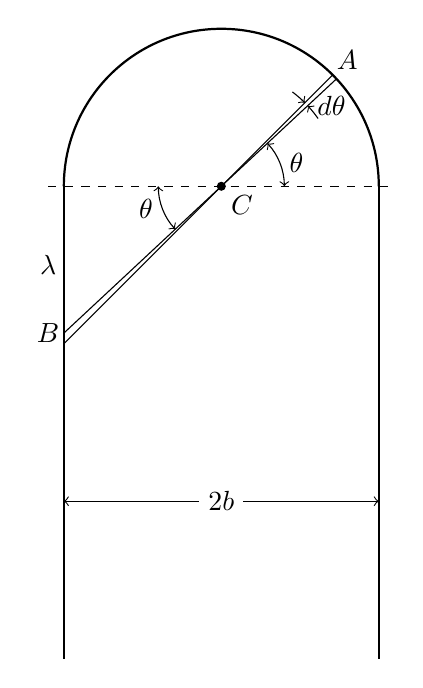
\begin{tikzpicture}
			% rods
			\draw[thick] (-2, 0) -- (-2, -6);
			\draw[thick] (2, 0) -- (2, -6);
			\draw[thick] (2, 0) arc (0:180:2);
			% labels and markers
			\node at (1.6, 1.6) {$A$};
			\node at (-2.2, -1.86) {$B$};
			\node at (-2.2, -1) {$\lambda$};
			\draw[<->] (-2, -4) -- (2, -4) node[midway, fill = white] {$2b$}; 
			\draw[dashed] (-2.2, 0) -- (2.2, 0);
			% point C
			\filldraw (0, 0) circle [radius = 0.05] node[anchor = north west] {$C$};
			% lines
			\draw (1.41421, 1.41421) -- (-2, -2);
			\draw (1.46271, 1.364) -- (-2, -1.86503);
			\draw[<->] (0.8, 0) arc (0:43:0.8) node [midway, right] {$\theta$};
			\draw[->] (1.22873, 0.860365) arc (35:43:1.5) node [right] {$d\theta$};
			\draw[->] (0.902723, 1.19795) arc (53:45:1.5);
			\draw[<->] (-0.8, 0) arc (180:223:0.8) node [midway, left] {$\theta$};
		\end{tikzpicture}
		\caption*{Figure 1.44}
	\end{figure}
	% Question

	\problemAnswer{
		\begin{enumerate}[label=(\alph*)]
			\begin{item}
				For element $A$, $dl=b\,d\theta$, and $dQ=\lambda b\,d\theta$. $dE=\frac{dQ}{4\pi\epsilon_0b^2}=\frac{\lambda\,d\theta}{4\pi\epsilon_0b}$.

				For element $B$, the radius is now $b/\cos\theta$. Because the length on rod has angle $\theta$ relative to the direction perpendicular to radius, $dl=b\,d\theta/\cos^2\theta$. so $dQ=\lambda b\,d\theta/\cos^2\theta$. $dE=\frac{dQ}{4\pi\epsilon_0(b/\cos\theta)^2}=\frac{\lambda\,d\theta}{4\pi\epsilon_0b}$.

				Therefore, the contribution of the two elements $A$ and $B$ has the same magnitude and opposite direction. They cancel each other. Field $\mathbf{E}$ vanished at point $C$.
			\end{item}
			\item Analogous to the one-dimensional setup, the field at point $C$ should add up to be zero.
		\end{enumerate}
	}
\end{homeworkProblem}

%----------------------------------------------------------------------------------------
%	PROBLEM 2
%----------------------------------------------------------------------------------------

\begin{homeworkProblem}
	(1.59) Zero field in a cylindrical shell

	Consider a distribution of charge in the form of a hollow circular cylinder, like a long charged pipe. In the spirit of Problem 1.17, show that the electric field inside the pipe is zero.
	% Question

	\problemAnswer{
		Consider two small circular patches on the cylindrical shell with radius $R$, defined by arcs projected from one point with the angle $d\theta$ onto the shell. One of them has the contribution to $\mathbf{E}$:
		\[
			dQ=\pi\left(\frac{r\,d\theta}{2}\right)^2\sigma
		\]
		\[
			dE=\frac{dQ}{4\pi\epsilon_0r^2}=\frac{(d\theta)^2\sigma}{16\epsilon_0}
		\]
		The other one has the contribution:
		\[
			dQ'=\pi\left(\frac{(R-r)\,d\theta}{2}\right)^2\sigma
		\]
		\[
			dE'=\frac{dQ'}{4\pi\epsilon_0(R-r)^2}=\frac{(d\theta)^2\sigma}{16\epsilon_0}
		\]
		They have the same magnitude, opposite direction, so they cancel each other. This explains why the electric field inside the pipe is zero.
	}
\end{homeworkProblem}

%----------------------------------------------------------------------------------------
%	PROBLEM 3
%----------------------------------------------------------------------------------------

\begin{homeworkProblem}
	(1.66) Force between two strips
	\begin{enumerate}[label=(\alph*)]
		\item The two strips of charge shown in Fig.~1.47 have width $b$, infinite height, and negligible thickness (in the direction perpendicular to the page). Their charge densities per unit area are $\pm\sigma$. Find the magnitude of the electric field due to one of the strips, a distance $x$ away from it (in the plane of the page).
		\item Show that the force (per unit height) between the two strips equals $\sigma^2b(\ln2)/\pi\epsilon_0$. Note that this result is finite, even though you will find that the field due to a strip diverges as you get close to it.
	\end{enumerate}
	\begin{figure}[H]
		\centering
		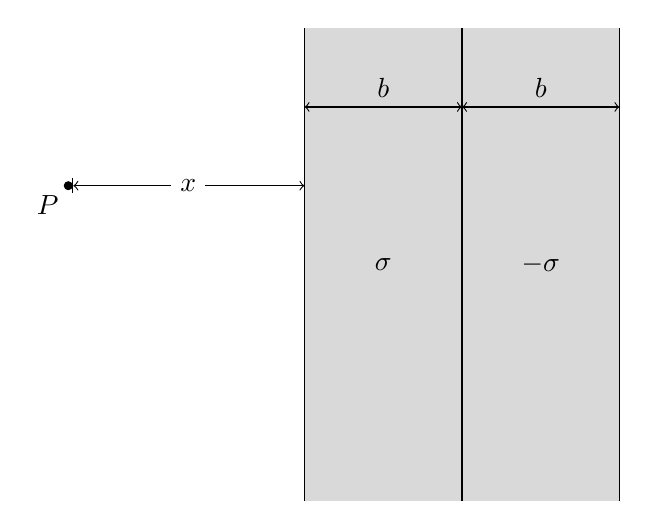
\begin{tikzpicture}
			\fill[gray!30!white] (-2, 1) rectangle (0, -5) node[black, midway] {$\sigma$};
			\fill[gray!30!white] (0, 1) rectangle (2, -5) node[black, midway] {$-\sigma$};
			\draw[<->] (-2, 0) -- (0, 0) node[midway, above] {$b$};
			\draw[<->] (0, 0) -- (2, 0) node[midway, above] {$b$};
			\draw (0, 1) -- (0, -5);
			\draw (-2, 1) -- (-2, -5);
			\draw (2, 1) -- (2, -5);
			\filldraw (-5, -1) circle [radius = 0.05] node[anchor = north east] {$P$};
			\draw[|<->] (-4.95, -1) -- (-2, -1) node[midway, fill = white] {$x$};
		\end{tikzpicture}
		\caption*{Figure 1.47}
	\end{figure}
	% Question

	\problemAnswer{
		\begin{enumerate}[label=(\alph*)]
			\begin{item}
			 	Consider a point $P$ on the left of the strips, distance $x$ away from the left edge of the strips, and consider the left strip only. Each vertical line of charge with width $dx$ contributes $E=\frac{\lambda}{2\pi\epsilon_0x}$ to the electric field, where its linear charge density could be obtained as $\lambda=\sigma\,dx$. The total $\mathbf{E}$ is:
			 	\[
				 	\int_{x+b}^x\frac{\sigma\,dx'}{2\pi\epsilon_0x'}=\frac{\sigma}{2\pi\epsilon_0}\int_{x+b}^x\frac{dx'}{x}=\frac{\sigma}{2\pi\epsilon_0}\ln\frac{x}{x+b}
			 	\]
			\end{item}
			\begin{item}
				A charge $dQ$ experience a force $\frac{\sigma\,dQ}{2\pi\epsilon_0}\ln\frac{x}{x+b}$ at a distance $x$. So a horizontal strip of charge on the other strip with charge density $-\sigma$ experiences force of:
				\[
					F=\int_0^b\frac{\sigma\,dQ}{2\pi\epsilon_0}\ln\frac{x}{x+b}dx=\frac{\sigma\,dQ}{2\pi\epsilon_0}b\ln4=\frac{b\sigma\,dQ}{\pi\epsilon_0}\ln2
				\]
				And $dQ$ is simply the charge density $\sigma$, neglecting directions. So the force is $\frac{b\sigma^2}{\pi\epsilon_0}\ln2$.
			\end{item}
		\end{enumerate}
	}
\end{homeworkProblem}

%----------------------------------------------------------------------------------------
%	PROBLEM 4
%----------------------------------------------------------------------------------------

\begin{homeworkProblem}
	(1.72) A plane and a slab

	An infinite plane has uniform surface charge density $\sigma$. Adjacent to it is an infinite parallel layer of charge of thickness $d$ and uniform volume charge density $\rho$, as shown in Fig.~1.50. All charges are fixed. Find $\mathbf{E}$ everywhere.
	\begin{figure}[H]
		\centering
		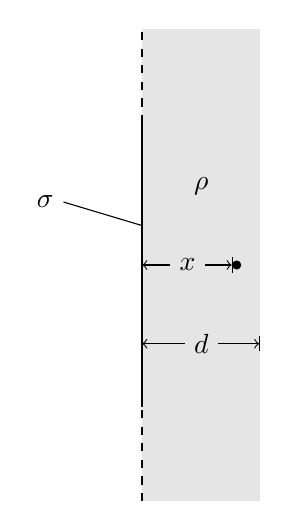
\begin{tikzpicture}
			\fill[gray!20!white] (0, 0) rectangle (1.5, 6);
			\draw[dashed, thick] (0, 0) -- (0, 1.2);
			\draw[thick] (0, 1.2) -- (0, 4.8);
			\draw[dashed, thick] (0, 4.8) -- (0, 6);
			\draw[<->|] (0, 2) -- (1.5, 2) node[midway, fill = gray!20!white] {$d$};
			\node at (0.75, 4) {$\rho$};
			\draw (0, 3.5) -- (-1, 3.8) node[anchor = east] {$\sigma$};
			\filldraw (1.2, 3) circle [radius = 0.05];
			\draw[<->|] (0, 3) -- (1.15, 3) node[midway, fill = gray!20!white] {$x$};
		\end{tikzpicture}
		\caption*{Figure 1.50}
	\end{figure}
	% Question

	\problemAnswer{
		For the infinite plane, the $E=\frac{\sigma}{2\epsilon_0}$.

		For the layer of charge, each layer with thickness $dx$ has the charge density $\rho\,dx$, and has the contribution to $E=\frac{\rho\,dx}{2\epsilon_0}$.

		For region to the left of the plane, the layer has
		\[
			E=\int_0^d\frac{\rho\,dx}{2\epsilon_0}=\frac{\rho d}{2\epsilon_0}
		\]
		So the $E=\frac{\sigma}{2\epsilon_0}+\frac{\rho d}{2\epsilon_0}$.

		For the region to the right of the plane, positioned $x<d$ from the plane, the layer has
		\[
			E=\int_0^x\frac{\rho\,dx'}{2\epsilon_0}=\frac{\rho x}{2\epsilon_0}
		\]
		from its left and $\frac{\rho(d-x)}{2\epsilon_0}$ from its right. The total $E=-\frac{\sigma}{2\epsilon_0}-\frac{\rho x}{2\epsilon_0}+\frac{\rho(d-x)}{2\epsilon_0}=-\frac{\sigma}{2\epsilon_0}-\frac{\rho x}{\epsilon_0}+\frac{\rho d}{2\epsilon_0}$.

		For the region to the right of the plane, positioned $x\geq d$ from the plane, similar to the region to left of the plane $E=-\frac{\sigma}{2\epsilon_0}-\frac{\rho d}{2\epsilon_0}$.

		The direction of $E$ would depend on the signs and magnitudes of $\sigma$ and $\rho$, but the positive direction is set to be to the left.
	}
\end{homeworkProblem}

%----------------------------------------------------------------------------------------
%	PROBLEM 5
%----------------------------------------------------------------------------------------

\begin{homeworkProblem}
	(1.83) Potential energy of a cylinder

	Problem 1.24 gives one way of calculating the energy per unit length stored in a solid cylinder with radius $a$ and uniform volume charge density $\rho$. Calculate the energy here by using Eq.~(1.53) to find the total energy per unit length stored in the electric field. Don't forget to include the field inside the cylinder.

	You will find that the energy is infinite, so instead calculate the energy relative to the configuration where all the charge is initially distributed uniformly over a hollow cylinder with large radius $R$. (The field outside radius $R$ is the same in both configurations, so it can be ignored when calculating the relative energy.) In terms of the total charge λ per unit length in the final cylinder, show that the energy per unit length can be written as $(\lambda^2/4\pi\epsilon_0)􏰔\left(1/4+\ln(R/a)􏰕\right)$.
	% Question

	\problemAnswer{
		\begin{equation}\tag{1.53}
			U=\frac{\epsilon_0}{2}\int_{\substack{\text{entire}\\\text{field}}}E^2\,dv
		\end{equation}
		The problem is equivalent to compressing charges from a disk of radius $R$ to a smaller disk of radius $a$.

		Outside the cylinder, the field at radius $r$ is $\frac{\lambda}{2\pi\epsilon_0r}$. Consider a disk with height $dh$ as shown below, whose $v=\pi r^2\,dh$, and thus $dv=2\pi r\,dr\,dh$. It holds charge of $\rho\pi a^2\,dh$, which means the linear charge density $\lambda=\rho\pi a^2$, when it is considered from its outside.
		\begin{figure}[H]
			\centering
			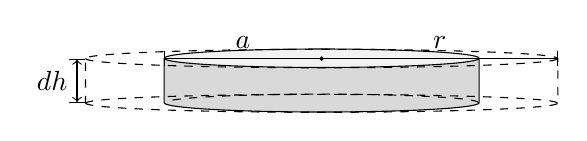
\begin{tikzpicture}
				\node[cylinder, draw = black, aspect = 1, minimum height = 0.8cm, minimum width = 4cm, shape border rotate = 90, cylinder uses custom fill, cylinder body fill = gray!30, cylinder end fill=gray!10] (B) {};
				\draw[dashed]
					let \p1 = ($ (B.after bottom) - (B.before bottom) $),
				        \n1 = {0.5 * veclen(\x1,\y1) - \pgflinewidth},
				        \p2 = ($ (B.bottom) - (B.after bottom)!.5!(B.before bottom) $),
				        \n2 = {veclen(\x2, \y2) - \pgflinewidth}
					in ([xshift = -\pgflinewidth] B.before bottom) arc [start angle = 0, end angle = 180, x radius = \n1, y radius = \n2];
				\node[cylinder, dashed, draw = black, aspect = 1, minimum height = 0.8cm, minimum width = 6cm, shape border rotate = 90] (A) {};
				\draw[dashed]
					let \p1 = ($ (A.after bottom) - (A.before bottom) $),
				        \n1 = {0.5 * veclen(\x1,\y1) - \pgflinewidth},
				        \p2 = ($ (A.bottom) - (A.after bottom)!.5!(A.before bottom) $),
				        \n2 = {veclen(\x2, \y2) - \pgflinewidth}
					in ([xshift = -\pgflinewidth] A.before bottom) arc [start angle = 0, end angle = 180, x radius = \n1, y radius = \n2];
				\draw[|<->|] ([xshift = -0.1cm] A.before top) -- ([xshift = -0.1cm] A.after bottom) node[midway, left] {$dh$};
				\filldraw ([yshift = -0.125cm] A.top) circle [radius = 0.02];
				\draw[-|] ([yshift = -0.125cm] A.top) -- ([xshift = 3cm, yshift = -0.125cm] A.top) node[midway, above] {$r$};
				\draw[-|] ([yshift = -0.125cm] A.top) -- ([xshift = -2cm, yshift = -0.125cm] A.top) node[midway, above] {$a$};
			\end{tikzpicture}
		\end{figure}
		The energy stored in the external field then is
		\[
			U_\mathrm{ext}=\frac{\epsilon_0}{2}\int_{r=a}^{r=R}\left(\frac{\rho\pi a^2}{2\pi\epsilon_0r}\right)^2 2\pi r\,dr\,dh=\frac{\rho^2\pi a^4}{4\epsilon_0}\,dh\int_a^R\frac{dr}{r}=\frac{\rho^2\pi a^4}{4\epsilon_0}\ln\frac{R}{a}\,dh=\frac{\lambda^2}{4\pi\epsilon_0}\ln\frac{R}{a}\,dh
		\]
		Inside the cylinder, also consider a disk with height $dh$ and radius $r$, whose $v=\pi r^2\,dh$, and thus $dv=2\pi r\,dr\,dh$. It holds charge of $\rho\pi r^2\,dh$, which means the linear charge density $\lambda=\rho\pi r^2$, when it is considered equivalently as a line charge.

		The energy stored in the internal field is
		\[
			U_\mathrm{int}=\frac{\epsilon_0}{2}\int_{r=0}^{r=a}\left(\frac{\rho\pi r^2}{2\pi\epsilon_0r}\right)^2 2\pi r\,dr\,dh=\frac{\rho^2\pi}{4\epsilon_0}\,dh\int_0^a r^3\,dr=\frac{\rho^2\pi a^4}{16\epsilon_0}\,dh=\frac{\lambda^2}{16\pi\epsilon_0}\,dh
		\]
		Therefore it is shown that the total energy for a disk of thickness $dh$ has the energy $\frac{\lambda^2}{4\pi\epsilon_0}\ln\frac{R}{a}\,dh+\frac{\lambda^2}{16\pi\epsilon_0}\,dh$. The energy per unit length is exactly
		\[
			\frac{\lambda^2}{4\pi\epsilon_0}\left(\frac{1}{4}+\ln\frac{R}{a}\right)
		\]
	}
\end{homeworkProblem}

%----------------------------------------------------------------------------------------

\end{document}
